\chapter{Le jeu Tétris}

\section{L'origine du jeu}

Tetris a été créé par Alekseï Leonidovitch Pajitnov au milieu des années 1980. Il était alors chercheur au centre informatique Dorodnitsyn de l'Académie des Sciences Soviétique, un laboratoire de recherche et développement de l'Union Soviétique. Il y travaillait à la reconnaissance de la voix humaine par les ordinateurs et, à ses heures perdues, s'amuser à programmer des jeux. 

\begin{center}
	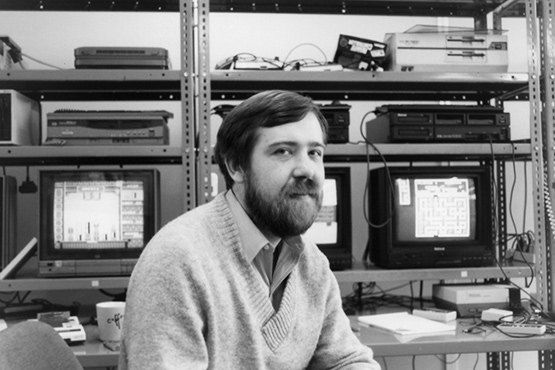
\includegraphics[scale=0.45]{../media/Pajitnov.jpg}
	
	Alekseï Pajitnov
	
	(Source: \url{http://allrus.me/legendary-russian-game-programmer-alexey-pajitnov/})
\end{center}

Il avait entendu parlé d'un puzzle créé par le mathématicien américain Salomon Golomb, le \textit{pentomino}, dont le but était de recouvrir un rectangle avec des pièces de différentes formes, toutes obtenues par l'assemblage de 5 carrés identiques.

\begin{center}
	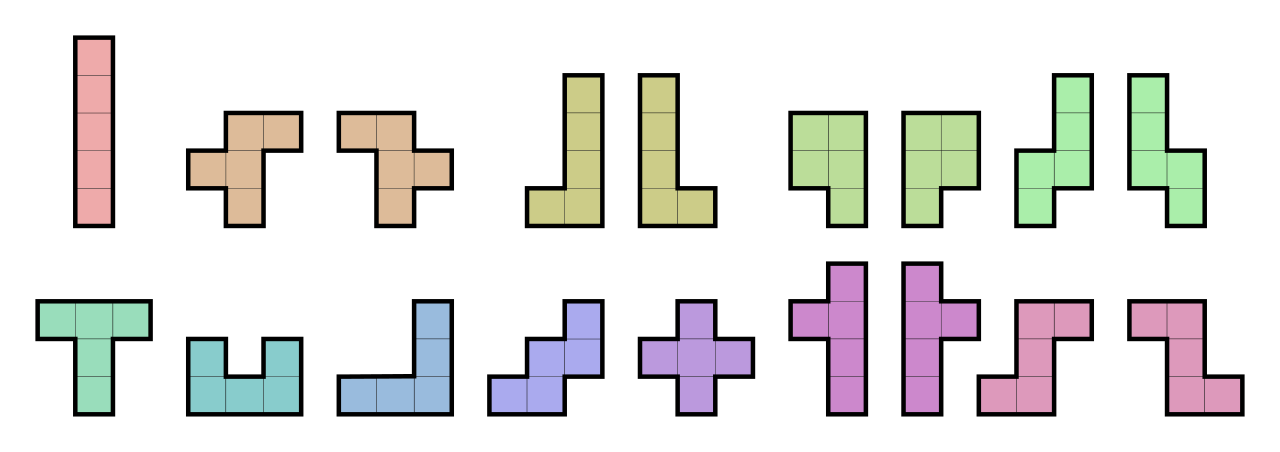
\includegraphics[scale=0.25]{../media/pentomino.png}
	
	Les 18 pièces du Pentomino (en distinguant les pièces symétriques)
	
	(Source: \url{https://fr.wikipedia.org/wiki/Pentomino})
\end{center}


Il s'en procura un et, commençant à y jouer, découvrit que, malgré les apparences, ce n'était facile du tout! Il eut alors l'idée d'en faire un jeu électronique dans lequel les pièces étaient choisies aléatoirement, l'une après l'autre, et à des intervalles de temps de plus en plus réduits. Il fit des tests mais devant le (trop) grand nombre de combinaisons qu'offraient les 18 pièces du pentomino, il décida d'opter pour une version simplifiée dans laquelle il n'y aurait que 7 types de pièces, toutes formées à l'aide de 4 carrés identiques. Ces pièces sont nommés les \og tétrominos \fg{}\footnote{On trouve aussi les appélations \og tétraminos \fg{} ou \og tétriminos \fg{}.}, du grec \textit{tetra} qui signifie \textit{quatre}. 

\begin{center}
	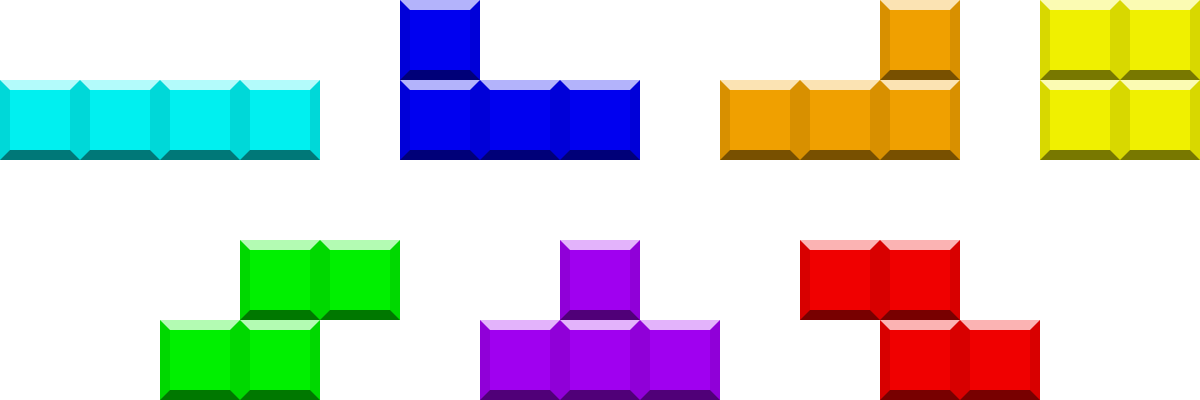
\includegraphics[scale=0.3]{../media/tetromino.png}
	
	\medskip
	
	Les 7 tétrominos: I, J, L, O, S, T et Z.
	
	(Source: \url{https://en.wiktionary.org/wiki/tetromino})
\end{center}

Le jeu fut développé sur un Elektronica 60. Cet ordinateur ne disposait pas de fonctionnalités graphiques et les carrés formant les pièces furent alors représentés par un espace encadré de crochets: $[~]$.

\section{Le principe du jeu}

Le principe du jeu est le suivant: dans un champ de jeu rectangulaire, une pièce est choisie aléatoirement parmi les 7 tétrominos et se déplace du haut vers le bas. Le joueur peut faire tourner d'un, deux ou trois quarts de tour et déplacer horizontalement dans les deux sens la pièce afin de disposer le tétromino comme il le souhaite en bas du champ de jeu, sachant que les pièces successives s'empilent les unes sur les autres. Lorsque le joueur parvient à recouvrir une ligne complète du champ de jeu à l'aide de carrés des tétrominos, sans qu'il n'y ait plus aucun trou sur la ligne, celle-ci disparaît, rapportant un certain nombre de points, et la pile de tétrominos est décalée vers le bas, laissant ainsi plus de place dans le champ de jeu pour accueillir les pièces suivantes. Si, à un moment, le champ de jeu ne contient plus assez de place pour accueillir le tétromino suivant, la partie est perdue! Ainsi, Tetris n'est pas un jeu dans lequel une partie se termine par la victoire du joueur. Il s'agit plutôt de faire le meilleur score possible.

\begin{center}
	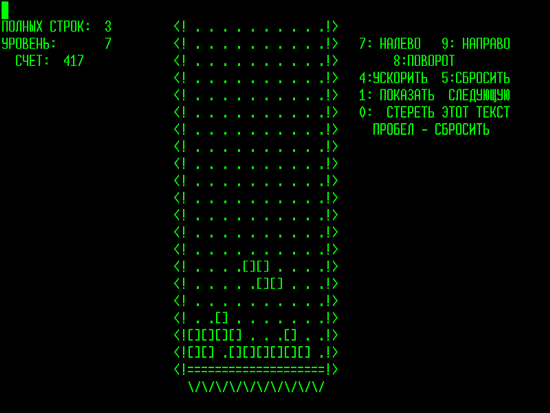
\includegraphics[scale=0.8]{../media/premiere_version.png}
	
	Première version de Tetris 
	
	(Source: \url{https://www.firstversions.com/2015/11/tetris.html})
\end{center}

\section{Diffusion du jeu}

Sentant que le jeu serait plus attractif si les tétrominos apparaissaient \og véritablement \fg{} à l'écran plutôt que leur représentation à l'aide des crochets, Pajitnov décida d'améliorer l'aspect visuel de son programme grâce à une version pour PC d'IBM intégrant une interface graphique. Pour cela, il fit appel à un jeune lycéen prodige de 16 ans, Vadim Gerasimov, qui lui avait été présenté par un autre programmeur du nom de Dmitri Pavlovsky. Gerasimov avait des compétences qui dépassaient largement celles de Pajitnov et Pavlovsky: il avait notamment appris seul à programmer dans un langage venu de l'Ouest: le Microsoft DOS. \`A l'issue de deux mois de travail, Gerosimov créa la première version \og couleur \fg{} de Tetris qui intégrait également une table des meilleurs scores programmée par Pavlovsky.  Selon Vadim Gerasimov, le nom Tetris résulte de la contraction des mots \og tetramino \fg{} et \og tennis \fg{}, ce dernier étant le sport favori de Pajitnov.


\begin{center}
	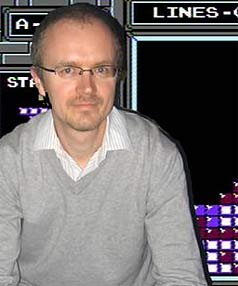
\includegraphics[scale=0.7]{../media/Gerasimov.jpg}
	
	Vadim Gerasimov
	
	(Source:   \url{http://www.stuff.co.nz/technology/games/2477794/Tetris-inventor-makes-waves-at-Google})
\end{center}

Cette version se diffusa rapidement d'abord à Moscou puis dans les pays de l'ancien bloc soviétique. Une copie fut envoyée par Victor Brjabrin, le supérieur de Pajitnov, à l'Institut des Sciences Informatiques de Budapest où Robert Stein, un anglais d'origine hongroise travaillant pour une société de logiciels, découvrit le jeu. Stein vit le potentiel du jeu et envoya un fax au centre informatique Dorodnitsyn pour indiquer qu'il était intéressé par Tetris. Pajitnov lui répondit simplement qu'il était également intéressé et, à partir de cette simple réponse, Stein se mit à exploiter et vendre les droits de Tetris auprès de diverses compagnies occidentales, sans avoir signé aucun accord avec les russes. Par la suite, il voulut établir un contrat en bonne et due forme avec Pajitnov et ses supérieurs mais ceux-ci étant confrontés à un monde inconnu pour eux, l'économie de marché, se montrèrent très méfiants et exigeants et les négociations n'aboutirent pas, ce qui n'empêcha pas Stein de continuer à exploiter Tetris. L'une des premières versions commerciales de Tetris fut celle éditée par Spectrum  Holobyte sur PC IBM en 1986. 

Par la suite, Elektronorgtechnica (abrégé ELORG), l'agence russe chargée de gérer les importations et exportations informatiques, repris le contrôle des négociations pour la gestion des droits et du marketing de Tetris, reprochant même à Pajitnov d'avoir donné un accord, fut-il de principe, à Stein, étant donné que, pendant l'ère soviétique, les créations intellectuelles des chercheurs russes étaient la propriété de l'état. Finalement, ELORG confirma l'accord avec Stein pour la gestion des droits de Tetris mais seulement sur les ordinateurs et à l'exclusion de tout autre matériel électronique. 

En 1989, les droits d'exploitation restants furent partagés entre Atari pour les bornes d'arcade et Nintendo pour les consoles. Minuro Arakawa, le président de la filiale américaine de Nintendo avait mandaté Henk Rogers, afin d'obtenir ces droits car il comptait faire de Tetris l'un des jeux phare de sa nouvelle console: la Game Boy. Celle-ci fut mise sur le marché en 1989 et connue un succès phénoménal avec des millions d'exemplaires vendus à travers le monde. Si les ventes de la Game Boy participèrent à la diffusion de Tetris, celui-ci contribua également au succès de la console car le jeu était, dans un premier temps, implanté d'office sur la machine.

\begin{center}
	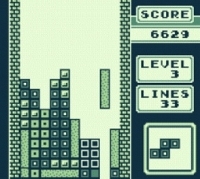
\includegraphics{../media/Tetrisgb.jpg}
	
	Le jeu Tetris sur Game Boy en 1989
	
	(Source: \url{ https://de.wikipedia.org/wiki/Liste_der_erfolgreichsten_Computerspiele})
\end{center} 

Par la suite, Nintendo développa différentes variantes du jeu puis, après de l'effondrement de l'URSS en 1991, Pajitnov émigra aux \'Etats-Unis et récupéra finalement l'intégralité des droits de Tetris en 1996. Il fonda avec Henk Rogers The Tetris Compagny qui a depuis la charge exclusive de la gestion des droits du jeu. Ainsi, Pajitnov, qui n'a touché aucun droit d'auteur durant plus de 10 ans, peut aujourd'hui récolter les fruits de sa création.

\section{Les raisons du succès}

Tetris possède deux caractéristiques qui en font un modèle de jeu vidéo et qui peuvent expliquer son succès: d'une part, il est facile à prendre en main mais, dans le même temps, il possède un côté addictif et, d'autre part, malgré son apparente simplicité, il ne peut exister que sur un support électronique. Le principe du jeu fait qu'il procure une satisfaction quasi immédiate puisqu'on arrive très rapidement à supprimer une première ligne, puis une deuxième, etc... Il fait partie de la famille des \og jeux occasionnels \fg{} (\textit{casual gaming}) car une partie ne demande pas un gros investissement en terme de temps et on peut y jouer quelques minutes puis arrêter pour refaire une partie plus tard sans n'avoir rien perdu de significatif. 

Le choix de Pajitnov de réduire le nombre de pièces à 7 est également un élément déterminant. En effet, 7 est le nombre d'\og objets\footnote{Il faut comprendre ici objet dans un sens très large: images, mot, idées, nombres, etc...} \fg{} différents que l'esprit humain peut mémoriser rapidement et sans trop d'effort alors qu'à partir de 8, cela devient beaucoup plus difficile. Ainsi, 7 est le nombre idéal de pièces puisqu'elles peuvent être mémorisées rapidement par le joueur. 

Enfin, la simplicité de son programme et le peu de ressources qu'il requiert lui a permis d'être développé sur tous les supports de jeu successifs (ordinateur, borne d'arcade, console, smartphone...) 

\section{Peut-on gagner à Tetris?}
La principale difficulté dans Tetris est l'accélération de l'arrivée des nouvelles pièces qui devient vite difficilement gérable. Il est clair que si cette accélération continue indéfiniment, on atteint un palier au-delà duquel le jeu n'est plus jouable, ne serait-ce que parce que le temps de déplacement de la nouvelle pièce devient inférieur au temps matériellement nécessaire pour la déplacer à l'aide des touches de la console ou de l'ordinateur. 

Imaginons qu'on mette de côté cet aspect du jeu et que les pièces arrivent à intervalle régulier. Dans ce cas, peut-on gagner à Tetris? Telle quelle la question n'a pas beaucoup de sens puisque le jeu ne prend fin qu'avec la défaite du joueur. Dans son mémoire de master, J. Brzustowski étudie la question sous l'angle suivant: existe-t-il une stratégie qui permette de jouer à Tetris indéfiniment. Il montre que cela dépend essentiellement du choix aléatoire des pièces. En particulier, il prouve que, quelle que soit la stratégie adoptée, il existe une suite de tetrominos S et Z qui conduit inéluctablement à la fin de la partie. 

Notons, cependant, que, dans le cas d'un choix au hasard des tetrominos, la probabilité qu'une telle suite sorte est très faible. De plus, Brzustowski met en évidence que le jeu n'est pas programmé pour faire perdre le joueur par le choix des tetrominos. C'est d'ailleurs le contraire puisque, dans la spécification officielle du jeu (\textit{Guideline}) disponible sur le site de The Tetris Compagny\footnote{\url{http://tetris.wikia.com/wiki/Tetris_Guideline}}, il est préciser qu'en fait les pièces sont choisies par vague de 7, une vague consistant en une permutation quelconque des 7 tetrominos: c'est le principe du \og sac aléatoire \fg{} (\textit{random bag}). Dans cette configuration, des stratégies gagnantes sont possibles mais Brzustowski constate également que face à la réalité du jeu (i.e. en tenant compte des contraintes temporelles), l'expérience acquise pas un joueur est plus efficace qu'une stratégie mathématique prédéfinie.




